\section{Progettazione Concettuale}


\begin{figure}[H]
    \begin{adjustwidth}{-2cm}{-2cm}
        \centering
        \label{fig:er-diagram}
        \caption{Diagramma Entità-Relazione}
        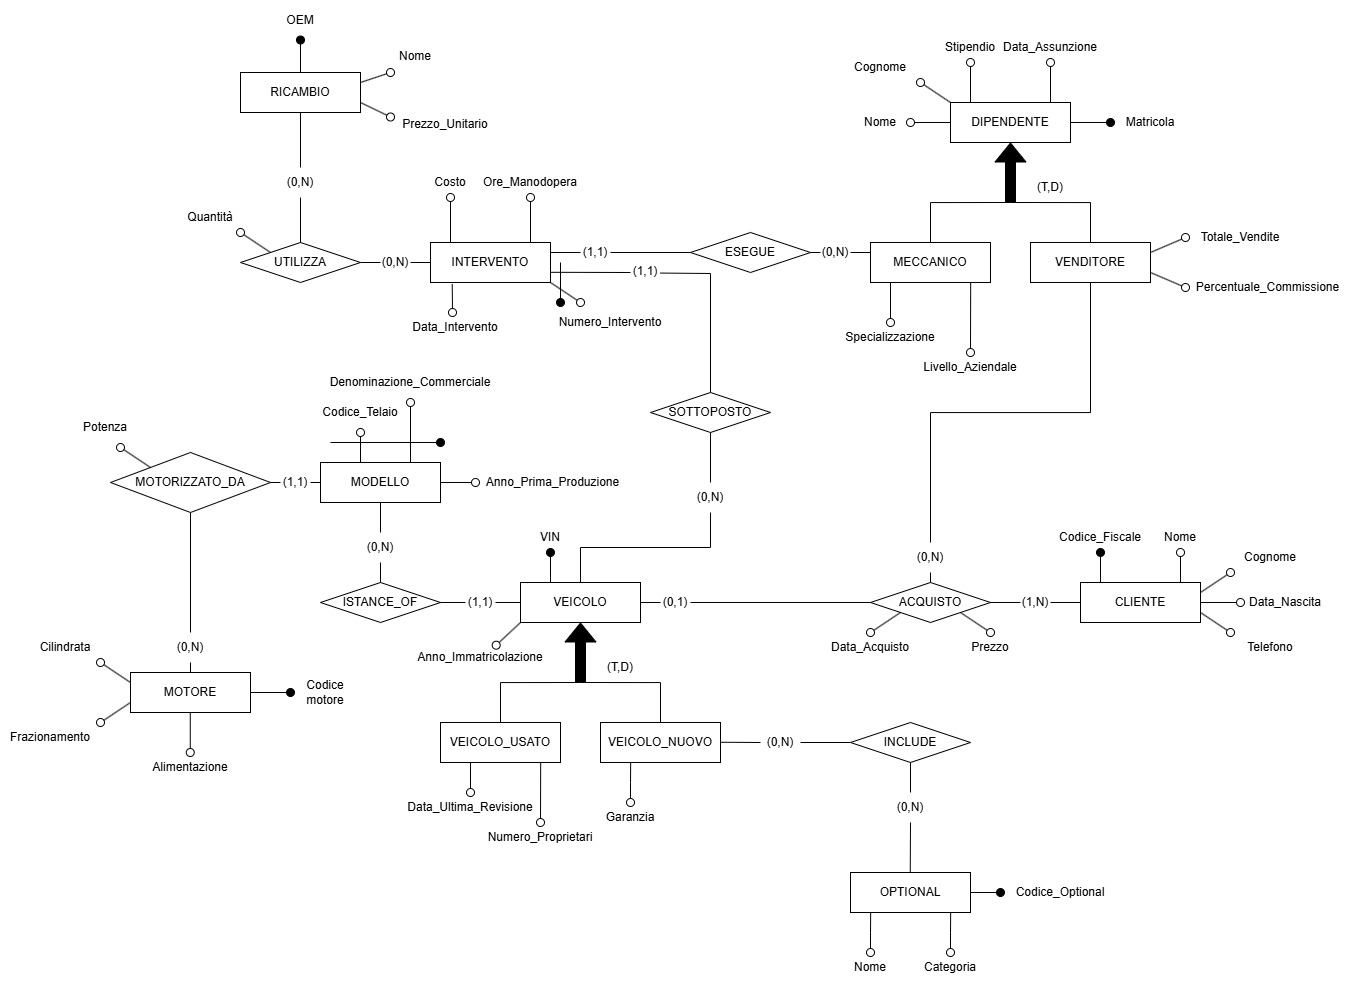
\includegraphics[width=1.25\textwidth, keepaspectratio]{allegati/Schema ER.jpg}
    \end{adjustwidth}
\end{figure}

La \textbf{Figura 1} mostra il diagramma Entità-Relazione (E-R) che riassume i requisiti descritti nella sezione precedente.

Esistono due tipologie di veicoli, nuovi e usati. Per i veicoli nuovi si vuole tenere traccia della garanzia e degli optional di cui dispongono, mentre per i veicoli usati vengono registrati il numero di proprietari precedenti e la data dell'ultima revisione.

Ogni veicolo è istanza di un determinato modello, il quale è a sua volta motorizzato da uno specifico motore. Per ogni associazione tra modello e motore viene inoltre registrata la potenza.

L'analisi dei requisiti pone particolare attenzione anche agli interventi effettuati sui veicoli. Ogni intervento si riferisce ad un solo veicolo ed è eseguito da un meccanico. Durante un intervento possono essere utilizzati uno o più ricambi, dei quali si vuole memorizzare anche la quantità impiegata.

Ogni acquisto coinvolge un cliente, un veicolo e un venditore, registrando inoltre la data e il prezzo della vendita. Un cliente può effettuare più acquisti nel tempo, mentre un determinato veicolo può essere associato al più ad un acquisto.

I dipendenti della concessionaria si distinguono in meccanici e venditori. Per i meccanici si vuole tenere traccia del livello aziendale e della specializzazione, mentre per i venditori vengono memorizzati il totale delle vendite effettuate e la percentuale di commissione.

Un venditore può non essere ancora associato ad alcuna vendita, così come un meccanico può non aver ancora eseguito interventi, al fine di consentire la registrazione nel sistema di dipendenti appena assunti.

La \textbf{Tabella 1} riassume tutte le entità e le relazioni individuate dall'analisi dei requisiti e rappresentate nel diagramma E-R, con i relativi attributi rilevanti. Per ciascuna entità viene inoltre indicato l'identificatore.

Il presente schema E-R non permette di rappresentare direttamente i seguenti vincoli:

\begin{itemize}
    \item Se un veicolo usato viene venduto, allora la \texttt{Data\_Acquisto} deve essere successiva alla \texttt{Data\_Ultima\_Revisione}.
\end{itemize}


\setlength{\tabcolsep}{6pt}
\renewcommand{\arraystretch}{1.7}
\setlength{\LTpre}{1.8cm}
\begin{longtable}{|p{2.5cm}|p{3.5cm}|p{5.8cm}|p{3cm}|}
\caption{\textbf{Descrizione delle entità del database}}
\label{tab:entita}
\\

\hline
    \multicolumn{1}{|c|}{\textbf{Entità}} &
    \multicolumn{1}{c|}{\textbf{Descrizione}} &
    \multicolumn{1}{c|}{\textbf{Attributi}} &
    \multicolumn{1}{c|}{\textbf{Identificatore}} \\
\hline
\endfirsthead

\hline
    \textbf{Entità} &
    \textbf{Descrizione} &
    \textbf{Attributi} &
    \textbf{Identificatore}
\\
\hline
\endhead

\hline
    Veicolo &
    Veicolo generico &
    \textit{VIN}, \textit{Anno\_Immatricolazione} &
    \textit{VIN}
    \\
\hline
    Veicolo\_Nuovo &
    Veicolo nuovo &
    \textit{Garanzia} &
    \textit{VIN} (ereditato)
    \\
\hline
    Veicolo\_Usato &
    Veicolo usato &
    \textit{Numero\_Proprietari}, \textit{Data\_Ultima\_Revisione} &
    \textit{VIN} (ereditato)
    \\
\hline
    Cliente &
    Cliente del concessionario &
    \textit{Codice\_Fiscale}, \textit{Nome}, \textit{Cognome}, \textit{Data\_Nascita}, \textit{Telefono} &
    \textit{Codice\_Fiscale}
    \\
\hline
    Dipendente &
    Dipendente generico &
    \textit{Matricola}, \textit{Data\_Assunzione}, \textit{Stipendio} &
    \textit{Matricola}
    \\
\hline
    Meccanico &
    Dipendente meccanico &
    \textit{Livello\_Aziendale}, \textit{Specializzazione} &
    \textit{Matricola} (ereditato)
    \\
\hline
    Venditore &
    Dipendente venditore &
    \textit{Totale\_Vendite}, \textit{Percentuale\_Commissione} &
    \textit{Matricola} (ereditato)
    \\
\hline
    Modello &
    Forma e dimensione del veicolo &
    \textit{Denominazione\_Commerciale}, \textit{Codice\_Telaio}, \textit{Anno\_Prima\_Produzione} &
    (\textit{Denominazione\_\allowbreak Commerciale}, \textit{Codice\_Telaio})
    \\
\hline
    Motore &
    Prodotto motore &
    \textit{Codice\_Motore}, \textit{Cilindrata}, \textit{Frazionamento}, \textit{Alimentazione} &
    \textit{Codice\_Motore}
    \\
\hline
    Optional &
    Prodotto opzionale del veicolo &
    \textit{Codice\_Optional}, \textit{Nome}, \textit{Categoria} &
    \textit{Codice\_Optional}
    \\
\hline
    Ricambio &
    Pezzo di ricambio &
    \textit{OEM}, \textit{Nome}, \textit{Prezzo\_Unitario} &
    \textit{OEM}
    \\
\hline
    Intervento &
    Intervento di officina &
    \textit{Numero\_Intervento}, \newline \textit{Data\_Intervento}, \textit{Ore\_Manodopera}, \textit{Costo} &
    \textit{Numero\_Intervento}
    \\
\hline
\end{longtable}



\setlength{\tabcolsep}{6pt}
\renewcommand{\arraystretch}{1.7}
\setlength{\LTpre}{1.8cm}
\begin{longtable}{|p{2.8cm}|p{5cm}|p{4.5cm}|p{2.5cm}|}
\caption{\textbf{Descrizione delle relazioni del database}}
\label{tab:relazioni}
\\

\hline
    \multicolumn{1}{|c|}{\textbf{Relazione}} &
    \multicolumn{1}{c|}{\textbf{Descrizione}} &
    \multicolumn{1}{c|}{\textbf{Componenti}} &
    \multicolumn{1}{c|}{\textbf{Attributi}} \\
\hline
\endfirsthead

\hline
    \textbf{Relazione} &
    \textbf{Descrizione} &
    \textbf{Componenti} &
    \textbf{Attributi}
\\
\hline
\endhead

\hline
    Acquisto &
    Acquisto di un veicolo da parte di un cliente assistito da un
    venditore &
    \textit{Cliente}, \textit{Veicolo}, \textit{Venditore} &
    \textit{Data\_Acquisto}, \textit{Prezzo}
    \\
\hline
    Sottoposto &
    Un veicolo viene sottoposto a
    un intervento &
    \textit{Veicolo}, \textit{Intervento} &
    \\
\hline
    Esegue &
    Un meccanico esegue un intervento &
    \textit{Meccanico}, \textit{Intervento} &
    \\
\hline
    Utilizza &
    Un intervento utilizza ricambi &
    \textit{Intervento}, \textit{Ricambio} &
    \textit{Quantità}
    \\
\hline
    Motorizzato\_Da &
    Un modello è equipaggiato 
    con un motore (con una certa potenza) &
    \textit{Modello}, \textit{Motore} &
    \textit{Potenza}
    \\
\hline
    Include &
    Un veicolo nuovo include optional &
    \textit{Veicolo\_Nuovo}, \textit{Optional} &
    \\
\hline
    Istance\_Of &
    Un veicolo è istanza di un modello &
    \textit{Veicolo}, \textit{Modello} &
    \\
\hline
\end{longtable}



\vspace{0.5cm}

Si noti che l'identificatore dell'entità \texttt{Intervento} include la relazione con un’altra entità.\newline
Infine, si noti che l'identificatore dell'entità \texttt{Modello} è un identificatore composto da due attributi.